\documentclass[10pt]{article}
%\usepackage[margin=1in]{geometry}
\usepackage{amsmath,amssymb,graphicx}
\usepackage{hyperref}
\usepackage{dirtytalk}
\usepackage{graphicx,float}
\usepackage{mathtools}
\setlength\parindent{0pt}
\usepackage[dvipsnames]{xcolor}

\usepackage{fancyvrb}

% redefine \VerbatimInput
\RecustomVerbatimCommand{\VerbatimInput}{VerbatimInput}%
{fontsize=\footnotesize,
 %
 frame=lines,  % top and bottom rule only
 framesep=2em, % separation between frame and text
 rulecolor=\color{Gray},
 %
 label=\fbox{\color{Black}data.txt},
 labelposition=topline,
 %
 commandchars=\|\(\), % escape character and argument delimiters for
                      % commands within the verbatim
 commentchar=*        % comment character
}



\begin{document}
\title{Assignment 4:  Parabolic Initial-Boundary Value Problem}
\author{1212550}
\begin{center}
\section*{Assignment 4:  Parabolic Initial-Boundary Value Problem}


The following is a brief report concerning the implementation of a C++ program to solve a specific instance of a Parabolic Initial-Boundary Value Problem (IBVP).\\
\end{center}

\section{The Problem}


In this assignment we will be considering an instance of a Parabolic IBVP, which is the Heat equation with diffusivity parameter $\kappa$:\\

\noindent\fbox{%
    \parbox{\textwidth}{%
Let $\kappa \in \mathbb{R}$. Solve the following for $u:I\times\Omega \rightarrow \mathbb{R}$,
\begin{align*}
u_t(t,x) &= \kappa u_{xx}(t,x) \quad (t,x) \in I \times \Omega \\
u(0,x) &= u_0(x) \\
u(t,x) &= 0 \quad (t,x) \in I \times \partial\Omega,
\end{align*}
where $ u_0 : \Omega \to \mathbb{R}$ is known.
    }
}\\

Specifically we we will be looking at solving
\begin{align*}
\begin{cases}
\partial_t u(x,t) = \kappa \partial_x^2 u(x,t) & (x,t) \in \Omega \times I, \\
u(x,0) = u_0(x) & x \in \Omega,
\end{cases}
\end{align*}
 where
\begin{align*}
u_0(x) =
\begin{cases}
0 & \text{if } x \leq \frac{1}{4} \text{ or } x > \frac{3}{4}, \\
1 & \text{otherwise}.
\end{cases}
\end{align*}

\subsection{The Method of Lines}

To do this we will be using the \emph{Method of Lines}, which first involves discretising in space. This will be done by applying the classical central difference
scheme for the Laplacian, with an equidistant spatial grid. The semidiscretisation generates an IVP for a system of ODEs:
\begin{align*}
\frac{dU_i}{dt} =
\begin{cases}
\partial^+\partial^-U_i \quad &\forall x_i \in \Omega_h, \\
U_i = 0 \quad &\forall x_i \in \Gamma_h.
\end{cases}
\end{align*}
These will be solved via Runge Kutta (RK) methods, which we encountered in the previous report. Specifically, we will be using the following three schemes:\\
\begin{itemize}
    \item Forward Euler (FE): $\quad$
\begin{center}
\begin{tabular}{ c|c }
  0 &    \\
  \hline
    & 1  \\
\end{tabular}
\end{center}

\item Backwards Euler (BE): $\quad$
\begin{center}
\begin{tabular}{ c|c }
  1 & 1   \\
  \hline
    & 1  \\
\end{tabular}
\end{center}

\item 3 stage Heun (Heun3):
\begin{center}
\begin{tabular}{ c|c c c }
  0 & & &   \\
  1/3 & 1/3 & & \\
  2/3 & 0 & 2/3 &  \\
  \hline
    & 1/4 & 0 & 3/4  \\
\end{tabular}
\end{center}
\end{itemize}

For completeness we recall the definition of RK methods\\

\noindent\fbox{%
    \parbox{\textwidth}{%
        $\textbf{Definition:}$ \textit{Runge-Kutta} methods are one-step methods of the form
\[
u_{n+1} = u_n + hF(t_n,u_n,f,h),
\]
where $F$ is defined as
\begin{align*}
    &F(t_n,u_n,f,h) = \sum_{i=1}^sb_iK_i, \\
    &K_i = f(t_n + c_ih, u_n + h\sum_{j=1}^sa_{ij}K_j), \quad i \in \{1, \dots, s \}.
\end{align*}
The integer $s$ denotes the number of stages of the method.\\
    }
}
\\

Note that in our case the $u_n$ are vectors and the function $f$ is a vector of central difference quotients.

\subsection{Implementation}

We aim to investigate the stability of the different schemes for various time-steps and spatial discretisations. Moreover, we aim to discuss the efficiency of these schemes. I have implemented header files \emph{models.hh} (along with models.cc) and \emph{scheme.hh}. The first contains a structure which defines the spatial discretisation of the problem. Note that along with defining the central difference matrix needed to define \say{$f$}, we also define its Jacobian. This is needed in order to use the Newton-Raphson method for calculating the $K_i$ for implicit RK methods. For the purposes of this assignment, it will only be used for the BE scheme. The latter header file includes a class \textit{DIRK} which defines a general RK method, and speific inhertience classes for the individual shcemes. The class also includes a function \textit{evolve} which updates the approximated solution at each time-step for a given scheme.\\


With these files in place, the included $\textit{main.cc}$ file allows the user to input the scheme, time step-size, spatial step-size and the diffusion parameter $\kappa$ via the terminal. The program is designed to compute the approximated solution and the results from this implementation will be considered in the next section.

\section{Testing}
In this section we run some tests on the implementation of the program.

\subsection{Stability}
For the following we have $\kappa$ fixed to be one. For the schemes FE and Heun3, one can see from the table below that we have a rough estimate for the maximum time step-size $\tau$ for various spacial step-sizes ($\frac{1}{N_x+1}$) i.e. for $\tau$ larger than these values, the schemes give an approximation which blows up. Unfortunately, for the BE scheme, the computation needs an excessive number of iterations to acquire a result for the cases $N_x =32$ and $64$.
\begin{center}


    \begin{tabular}{|c||c|c|c|}
    \hline
        $N_x$:      & 16 & 32 & 64 \\
    \hline
       \hline
       estimate - max $\tau$ for FE  & 0.001 & 0.0004 & 0.0001    \\
       \hline
       estimate - max $\tau$ for BE  & 0.0008  & N/A& N/A  \\
        \hline
       estimate - max $\tau$ for Heun3 & 0.001 & 0.0004 & 0.0001 \\
       \hline
    \end{tabular}
\end{center}
In particular we note that this agrees with the \emph{Courant-Friedrichs-Levy} condition, which says we necessarily obtain a limit on the temporal stepsize as $\tau \leq Ch^2$ for some constant $C>0$. If we choose 5 equidistant points in time, $t_n = \frac{nT}{5}$ ($n \in \{1, \dots, 5\}$), it can be seen that the for each fixed $t_n$ the solution increases to begin with, and later descends as the spatial parameter $x$ increses from 0 to 1. This can be seen more clearly in the graphs included at the end of this report (considered for the cases where $\tau = 0.0002$, $\kappa = 2$, $N_x = 32$ and  $\tau = 0.001$, $\kappa = 1$, $N_x = 16$ for the FE scheme.

\subsection{Efficiency}
The FE and Heun3 schemes are far more efficient than the BE scheme. This is dude to the fact that the latter is the only implicit scheme and thus (in my implementation) uses the Newton-Raphson method to calculate the $K_i$. This involves using the Gauss-Seidel algorithm at each iteration, which is costly. For example, even for $\tau = 0.001$, $N_x = 50$ and $\kappa = 1$, the Heun3 scheme is computationally faster than BE at  $\tau = 0.0001$, $N_x = 16$ and $\kappa = 1$.

 \begin{figure}[H]
 \begin{center}
    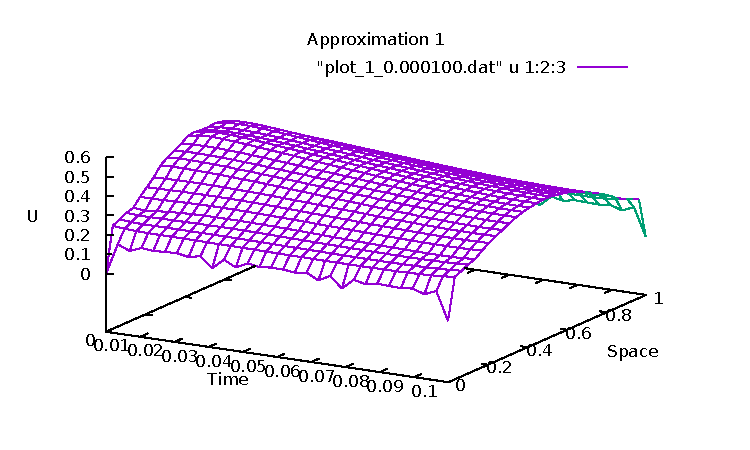
\includegraphics[width=1\textwidth]{plot1.pdf}
  \end{center}
  \caption{Test 1: time-step $\tau = 0.0001$, $N_x = 16$ and $\kappa = 1$
  \label{fig:2_01}}
\end{figure}

 \begin{figure}[H]
 \begin{center}
    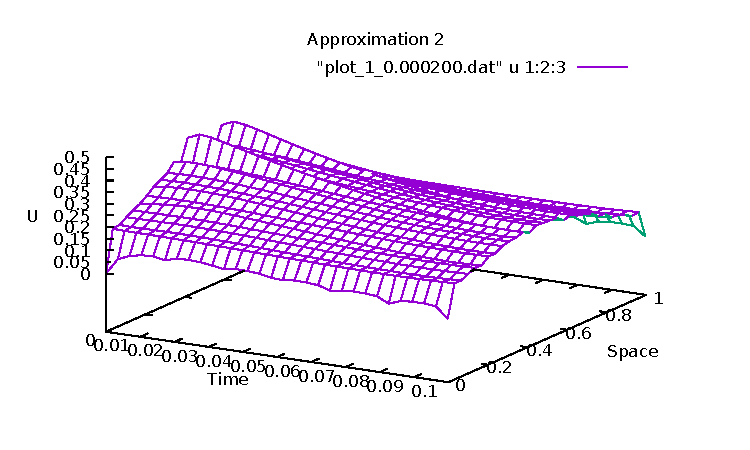
\includegraphics[width=1\textwidth]{plot2.pdf}
  \end{center}
  \caption{Test 2: time-step $\tau = 0.0002$, $N_x = 32$ and $\kappa = 2$
  \label{fig: 2_001}}
\end{figure}

\end{document}
